\chapter{Making Decisions} 

\section{Introduction} 

At the end of the previous chapter we saw how we could get the user to type something in, and then advance the story. In this chapter, we explore this further. We start with the user simply pressing \emph{Enter} to advance the story, just like turning a page. Then, we look at \textit{variables}, for example \textit{String} variables that can hold text. We use a variable to pick up what the player just typed in -- remember \texttt{command}? Once we have that, we inspect what the player wants to do (e.g. look around, or go south) and drive the story forward accordingly. For that, you learn more about the \texttt{if..then..else} control structure in Python, and basic String comparison \texttt{==}. By the end of the chapter, we will have a game where the player can roam around various rooms in the house, look around, and find all manner of horrific things ... 

\section{The Story So Far} 

So far, the story is that you are in "a dark, spooky house, all alone out in the forest." Scary thing is, you are inside -- and you cannot get out! Whereas, hearing strange noises, getting out is clearly what you want ... 

 \begin{Gmd}[Victory condition] Most games have a \textit{\victorycondition}: What you need to achieve to win the game. Collect all the little shiny boxes, like in \emph{Fez}, or defeat all the monsters, like in \emph{Dark Souls}, or free the princess in \emph{Super Mario}. (Not all games have apparent victory conditions, for example look at an exploration game like \emph{Dear Esther}.) Key is of course that the player has some idea about what the victory condition might be. In our story, the first few lines already make it clear: Escape! Which then turns into the question, how ....  \expend  
  \end{Gmd} 
  
  Having some idea about what you need to achieve is good, but even better is knowing \emph{how} you can achieve it! This is where \gamemechanic{s} and \event{s} come into play (literally).   
      
  \begin{Gmd}[Game mechanics and events] A \textit{\gamemechanic} defines how the game works. It is a rule we implement in code, determining what a player can do. If the player does "this," then "that" is going to happen. For example, many games use the \emph{A} button on the (Xbox) controller to make your character jump. That is a mechanic. Or, in text adventures, you type in a command -- that is another mechanic. When you are playing a game, you use these mechanics to make things, \textit{\event{s}}, happen. Things may go one way or the other, depending on what you decide to do. Take again \emph{Dark Souls} -- as the monster attacks you, do you press \emph{L1} to raise your shield and block the attack, or do you use your left stick and \emph{O} to roll to the side? Different mechanics, allowing you to take different actions, resulting in different ways in which the game might play out ...   \expend
  \end{Gmd}
  
Let's use that to work out our story a little bit more. The \victorycondition\ is to get out of the house but the only door outside is locked. Let's assume that that means the player needs to find a key. As the game wouldn't be particularly exciting if the key would be laying there right in front of the player's nose, we need some \gamemechanic{s} for the user to go around the house, and look for objects. And that should, of course, lead to some "interesting" events ...  

\begin{figure}[h]
\centerline{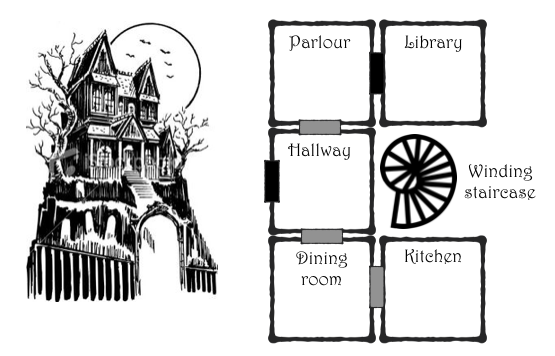
\includegraphics[scale=.70]{images/p1ch2-hauntedhousemap.png}}
\caption{The Haunted House In The Forest}\label{fig:hauntedhousemap}
\end{figure}

\figref{fig:hauntedhousemap} shows the map of the house. The black and grey triangles indicate doors. Grey means the door is open, black means that door is closed. The player needs to find the right key to open a closed door. The player can find the key to the \emph{Library} in the \emph{Parlour}. The key to the door outside is in a handbag in the \emph{Kitchen}. 

Now, this would not be a scary story if there would not be any monsters around ... So let's place a Ghoul in the kitchen, to guard the Key To Outside. This is going to be our \emph{Boss Fight}! 

We should not allow the user to simply waltz into the kitchen, completely ignore the Ghoul, and just grab the key. No -- if the player does that, "You Died!" Instead the player needs to find a weapon to defeat the Ghoul. The Library is a good place for that. We can put a sword above the mantelpiece. For good measure we also put a Ghost in the Library. The Ghost floats in front of the sword. 

Those are our key objects: the key to get into the Library (found in the Parlour), the sword to kill the Ghoul (found in the Library), and the key to get out of the house . The player can find that final key in a handbag in the Kitchen. To spice things up, we can let the Ghoul carry the handbag around its neck.  

We now have our locations, our objects, a monster -- what we need now still is define what the player can do. 

We have objects, so a player should be able to \textbf{take} an object -- "take sword" or "pick up key." 

We are not going to place these objects in plain sight, as that would be too easy. The player should \textbf{search} -- "search room" or "look in handbag." 

Naturally, the player needs to be able to get around the house. We can do that "old school"-style using \textbf{go} with a compass direction -- "go north", "go south." From the Hallway you can go North to the Parlour, or South to the Dining Room, etcetera. 

Finally, as we have monsters, the player needs to be able to \textbf{attack} a monster -- or \textbf{retreat} if the monster is too scary! 

Okay, there we go. All we need now is the story ... and the code. 

\section{Getting The Story Going} 

Let us have a look again at the code we have so far. 

\begin{lstlisting}
print("You are in a dark, spooky house, all alone out in the forest.")
print("There is only one door to the outside, and it is locked.")
print("You hear strange, creaky sounds.")
command = input("> ")
print("Boo!")
\end{lstlisting}

As our story is going to continue well beyond the cheap jump scare in line 5, we can delete the "Boo!" Instead, we should take stock of the situation. What do we know? Well, we know that the player does \emph{not} have the main key, nor the key to the library, nor the sword -- nor the handbag for that matter. All of that is key to achieving the victory condition: 

\begin{enumerate}
\item Search the Parlour to find the key to the Library
\item In the library, attack the Ghost, then take the sword
\item In the kitchen, use the sword to attack the Ghoul
\item After the Ghoul has been defeated, take the handbag
\item Search the handbag, find the main key
\end{enumerate} 

Once the player has the main key, he should go to the Hallway, and escape the haunted house. Game over, "You Win!"

This means we need to track what the player already has. We can use variables for that. A variable is essentially a "container" you can put a value in (assign a value to). For example, look at line 4 again: 

\begin{verbatim}
command = input("> ")
\end{verbatim}      

We introduce here a variable \texttt{command}, to which we assign a value we get from the function \texttt{input} -- i.e. command stores what the user has just typed in. In Python, there are various types of variables. The \texttt{command} variable is a variable of type \textit{\strvar}. A \strvar\ stores text. If the user types in \textit{go south} and presses enter, then the \emph{value} of \texttt{command} becomes 'go south'. 

\begin{Exe} 
Try this out in \texttt{idle}. Type line 4 in \texttt{idle}, and then type in a command. After you have pressed enter, type in \texttt{command} (the variable name), and press enter again. \texttt{idle} shows the value assigned to that variable.  \expend
\end{Exe}

There are also various other types of variables. Two types you will frequently encounter are \textit{\integer} variables, and \textit{\boolean} variables. An \integer\ variable stores (whole) numbers. 

 \begin{Exe} 
Try this out in \texttt{idle}. Type in \texttt{score = 0}. You have zero points! To check that, type in \texttt{score} (and press enter), and you will see -- 0. If you want a higher score than that, simply add that to the variable, like so: \texttt{score = score + 100}. This means, "take the current score, add 100, and store the resulting number again in score." Now add another 10 points, and check what value is assigned to \texttt{score}. \expend
\end{Exe}

\begin{Exp}[Integer addition short cut] 
If all you want to do is add a number to the current value of an \integer\ variable, and assign the result again to that variable, (like we did above), then Python has a shortcut for that. Instead of \texttt{score = score + 100} you can also use the short-cut \texttt{score += 100}. \expend
\end{Exp} 
 
A \boolean\ variable is a variable that is either \texttt{True} or \texttt{False}. We can use such variables to track whether the player has certain items. Does the player have the sword? The main key? At the beginning -- none of that, so we set all those variables to \texttt{False}. 

We often call such \boolean\ variables "\flag{s}"  A flag variable is a variable you define to have one value until some condition is true, in which case you change the variable's value. For example, \texttt{hasSword = False} until the player has taken the sword in the Library -- then it becomes \texttt{True}.  It is a variable you can use to control the flow of a function or statement, allowing you to check for certain conditions. So, only once it is the case that \texttt{hasSword = True}, the player can attack the Ghoul and stand a chance to survive that encounter. 

Type in the code below, before the first \texttt{print} line. Something new: Lines 1 and 6 start with \texttt{\#}. This indicates a comment; Python happily ignores those lines. Note that you do not need to retype all the print statements; the full code listing is included for illustration. 

\begin{lstlisting}
# Initialize flags 
hasMainKey = False 
hasHandbag = False
hasSword = False 
hasLibraryKey = False 
# The story begins -- the Hallway
print("You are in a dark, spooky house, all alone out in the forest.")
print("There is only one door to the outside, and it is locked.")
print("You hear strange, creaky sounds.")
command = input("> ")
\end{lstlisting}

What is the first thing that the player might do in such a situation, other than scream "lemme out!?!"? Well, either of two things. Either the player indeed says "help," or something like "look around." If the player says "help", we can help him (or her) out by saying some soothing words, and briefly explain what actions can be performed. Type in the code below. After the code we explain what this new \texttt{if..} construction means.   

\begin{lstlisting}[firstnumber=last]
if (command == "help"):
    print("Don't be scared. You can do a couple of things:")
    print("- 'go' in a compass direction, e.g. 'go south' ")
    print("- 'search' to 'search room', or look into an object")
    print("- 'attack' to attack a monster")
    print("- 'take' an object, e.g. 'take key' ")
\end{lstlisting}

The \texttt{if} statement in line 11 is a check. If the player typed in \textit{help}, then do whatever comes after the \texttt{:} -- in this case, several print statements. For Python it is very important that the block of code that should be executed, is properly \textit{indented}. As you can see, the \texttt{print} statements do not begin at the same position as the \texttt{if} position, but a little further. Atom does this automatically. 

Another thing you may notice is that we use a double "==" and not a single "=" to make a check. This is important, and makes all the difference. A single "=" \emph{assigns} a value to a variable -- a statement \texttt{score = 10} assigns the value 10 to the variable \texttt{score}. A double "==" compares the value of the variable, to the value provided. So, \texttt{score == 10} is a check whether the score is 10 (or not) -- or, as in line 11, we check whether the player's command was "help."   

\begin{Exp}[Single or double quotes?] 
Finally, once we are talking about things you may be noticing: When you used \texttt{idle} to check the value of a \strvar\ variable, the value was returned with single quotes, e.g. \texttt{'help'}. But now, line 11 is using double quotes -- \texttt{"help"}! Why, what is the difference? Simple answer: There is no difference. You can use double quotes or single quotes, and to Python it is all the same. In general, we use double quotes here, and in lines 12 through 16 you also see we are using single quotes inside double quotes ... not a problem. \expend 
\end{Exp}

The following code provides the player with more details about the Hallway, should he be looking around. Looking at the map in \figref{fig:hauntedhousemap} (on p.\pageref{fig:hauntedhousemap}) again, we see that the player has several possibilities. 

\begin{lstlisting}[firstnumber=last]
 if (command == "look around"):
    print("You find yourself in the hallway.")
    print("To the east is a winding staircase, on the verge of collapse.")
    print("To the west is the door to the outside.")
    print("You can go north, and south.")
\end{lstlisting}

Before we let the player go to the Parlour, let's handle the case where somebody is really scared and desperately wants to get out of this house as fast as possible. What if the player says \texttt{go west}? Well, if the player has the main key -- fine, go ahead, you win. But if not ... So what we need to do, after checking whether the command is \texttt{go west}, is what the status of our \texttt{hasMainKey} flag is. No key? No exit. 

\begin{lstlisting}[firstnumber=last]
if (command == "go west"):
    if (hasMainKey == True) :
        print("You have escaped the house! You can breathe easy now.")
    else:
        print("The door is locked. You need a key...")
\end{lstlisting}

Line 23 checks whether the player has the key. If that is the case (\texttt{hasMainKey == True}), then the player wins. If that is \emph{not} the case, then we get to the \emph{else} statement in line 25. Note that this other case means \texttt{hasMainKey} is \texttt{False}, as a \boolean\ can only have one of these two values. The player is informed that he cannot go ("oh nooooo.....") but he does get a little hint: go look for the key ... 

\begin{Exe}
Run the program in the terminal. Type in a command. What happens, after you have typed in the command? \expend
\end{Exe}

(In case you read this already without doing the exercise first -- no cheats or shortcuts!) Indeed. After you have typed in a command (help, look around, go west), the program ends. That's not much of an adventure of course, so we should change that. Add another statement \texttt{command = input("> ")} at the end of the long \texttt{print} blocks for "help" and "look around", and at the end of the "else" block (after line 26). Make sure to use the right indentation!  
      
\begin{Exe}
Run the program in the terminal. Type "help." After that, try "look around." Does that work? Now try "go west." What happens if you \emph{now} type in "look around"? Can you explain why?\footnote{The answer: We go step-by-step through the program, and in this program you cannot go back. So once you are passed "look around" the only next step you can take is "go west" as the program no longer checks for "help." Not great, indeed, but it's a start. Later on we will see how to do better.} \expend
\end{Exe}

It's time to get the player moving around. First, we go north, to the Parlour. There the player can find the key to the Library, and once we are in the Library, there is a Ghost to deal with before the player can then take the sword ... 

\begin{lstlisting}[firstnumber=last]
if (command == "go north"):
    print("You go through the door, into the Parlour.")
    print("Heavy curtains cover most of the windows. ")
    print("It smells dusty here.")
    print("There is a door to the west, which appears locked.")
    command = input("> ")
    if (command == "look around" or command == "search room"):
        print("In the faint light, you see several chairs, and a coffee table.")
        print("A key is laying on the coffee table.")
        command = input("> ")
    if (command == "take key"):
        hasLibraryKey = True
        print("You found the key to the library!")
        command = input("> ")
\end{lstlisting}
 
Once you have typed in the code above, let's have a closer look. 

First of all, notice the \texttt{or} in line 33. This means: if the player typed in \emph{either} "look around" \emph{or} "search room", execute the block of code after that. So we offer the player a little bit of flexibility here in how he can phrase what he wants to do. 

\begin{Exe}
If you like, you can go back and change the code in line 17, to match line 33. \expend 
\end{Exe}

Another thing is that we are starting to change our flags. Assuming the player has seen there is a key, and then decided to "take key" we can now set the flag \texttt{hasLibraryKey} to \texttt{True}. 

Alright, so now the player has the key to the library. If the player now says, "go west" -- no problem. Or, if the player has not looked around so far, and thus does not know there is a key to pick up, then "go west" should not take him into the Library. Just like we saw in line 23, we can check our flags, and handle that too. 

Or so it seems ... but first things first. 










  